% ------------------------------ INICIO Paquetes ----------------------------- %

\documentclass[conference]{IEEEtran}
\IEEEoverridecommandlockouts
% The preceding line is only needed to identify funding in the first footnote.
%If that is unneeded, please comment it out.
\usepackage{cite}
\usepackage{amsmath,amssymb,amsfonts}
\usepackage{algorithmic}
\usepackage{graphicx}
\usepackage{textcomp}
\usepackage{xcolor}
\usepackage[utf8x]{inputenc}
\def\BibTeX{{\rm B\kern-.05em{\sc i\kern-.025em b}\kern-.08em
    T\kern-.1667em\lower.7ex\hbox{E}\kern-.125emX}}

\usepackage{url}
%\usepackage[font=small]{caption}

% ------------------------------- FIN Paquetes ------------------------------- %

\def\contentsname{Contenidos}
\def\listfigurename{Lista de Figuras}
\def\listtablename{Lista de Tablas}
\def\refname{Referencias}
\def\indexname{Índice}
\def\figurename{Fig.}
\def\tablename{TABLA}
\def\partname{Parte}
\def\appendixname{Apéndice}
\def\abstractname{Resumen}
\def\IEEEkeywordsname{Palabras clave}

\begin{document}
	
% Para modificar estilo de bibliografía y forzar el uso de "et al." cuando hay 6 autores o más
% NO QUITAR
\bstctlcite{IEEEexample:BSTcontrol}

% ------------------------------ INICIO Portada ------------------------------ %

\title{
	Análisis de Sentimientos en texto mediante SVM y Redes Neuronales Convolucionales
}

\author{
    \IEEEauthorblockN{Jhonathan Daniel Abreu Luque}
    \IEEEauthorblockA{
    	\textit{Escuela de Ingeniería de Sistemas}\\
    	\textit{Universidad de Los Andes}\\
    	Mérida, Venezuela\\
    	jd.abreu25@gmail.com
    }
}

\maketitle

% -------------------------------- FIN Portada ------------------------------- %

% ---------------------------------------------------------------------------- %

% ------------------------------ INICIO Resumen ------------------------------ %

\begin{abstract}

	Las emociones son un componente semántico primario en la interacción humano-humano y juegan un papel sumamente importante en el comportamiento humano. Por tal motivo, la presente investigación se enfoca en el estudio de diferentes técnicas de representación numérica de documentos de texto y de clasificación de los mismos en base al sentimiento de evocan. Se comparan dos técnicas de vectorización, Word2Vec y el modelo clásico Bag-Of-Words para preparar la data que alimenta a clasificadores de tipo SVM y Redes Neuronales Convolucionales. Los datos utilizados para el entrenamiento y prueba fueron recolectados como parte de la investigación. Los resultados del estudio muestran que, para cantidades pequeñas de datos, modelos sencillos de vectorización, como Bag-Of-Words, se desempeña mejor que otros más complejos. Los clasificador que generó los mejores resultados fueron las Redes Neuronales Convolucionales, sobre todo cuando se toma en cuenta mayor cantidad de información contextual en el proceso de vectorización de los documentos.

\end{abstract}

% -------------------------------- FIN Resumen ------------------------------- %

% ---------------------------------------------------------------------------- %

% --------------------------- INICIO Palabras clave -------------------------- %

\begin{IEEEkeywords}
	
	Análisis de sentimientos, vectorización, clasificación, Redes Neuronales Convolucionales, SVM, Bag-Of-Words.
    	
\end{IEEEkeywords}

% ----------------------------- FIN Palabras clave --------------------------- %

% ---------------------------------------------------------------------------- %

% ---------------------------- INICIO Introducción --------------------------- %

\section{Introducción}

    Imagina un mundo en el que los humanos solo tengan las palabras como medio de comunicarse; un mundo en el que las expresiones faciales y corporales no jueguen ningún papel en la expresividad de las personas. Ahora intenta ponerte en el lugar de aquellas personas que viven con limitaciones motoras y cognitivas que les impiden expresar lo que piensan y sienten más allá de las palabras.

    Las emociones son un componente semántico primario en la interacción humano-humano y juegan un papel sumamente importante en el comportamiento humano. Las emociones, al igual que el pensamiento, guían las acciones y los diálogos. Es por esto que una de las aplicaciones de gran importancia que puede darse al análisis de sentimiento es la robótica social, en la que se necesitan robots que sirvan como extensiones para los cuerpos de las personas con limitaciones motoras que les impidan expresarse por canales diferentes al habla; módulos que permitan a los robots detectar las emociones de los usuarios, de modo que puedan responder a los mismos y adaptarse a la interacción; robots que puedan expresar emociones para generar empatía. Sin embargo, no es el único campo de acción de esta disciplina.
    
    Analizar la creciente cantidad de reseñas de productos permitiría a las empresas detectar potenciales clientes y sus preferencias; analizar reseñas de películas permitiría la automatización de la clasificación de grandes bases de datos de cine internacional; detectar el sentimiento de una conversación permitiría que los avatares en juegos en linea muestren emociones en tiempo real, aumentando así la expresividad de las conversaciones humanas, incluso en ámbitos sociales remotos. Estas y muchas otras áreas forman el amplio campo de aplicación del análisis de sentimientos.
    
    El presente artículo pretende sentar las bases para el desarrollo de un framework de detección de emociones de texto para una futura integración en un avatar robótico, de modo que se vea dotado de nuevos canales de expresión e interactividad. Para esto, se requiere analizar métodos de representación de las oraciones de modo que puedan ser alimentadas a un clasificador y, además, realizar un estudio comparativo que permita detectar el clasificador más apto para este fin entre las SVM y las Redes Neuronales Convolucionales.
    
    El resto de este articulo, entonces, se organiza de la siguiente manera: en la Sección \ref{sec:antecedentes} se presenta el trabajo relacionado que ya ha sido realizado en el área del análisis de sentimientos de texto. La Sección \ref{sec:metodologia} describe la metodología utilizada, con una breve introducción a los vectorizadores y los clasificadores a estudiar. La Sección \ref{sec:experimentos} muestra las pruebas realizadas y el análisis de los resultados obtenidos. Por último, la Sección \ref{sec:conclusiones} presenta las conclusiones dela investigación y los pasos siguientes para la continuación del proyecto.

% ----------------------------- FIN Introducción ----------------------------- %

% ---------------------------------------------------------------------------- %

% ------------------------- INICIO Trabajo Relacionado ----------------------- %

\section{Trabajo Relacionado} \label{sec:antecedentes}

    El análisis de sentimientos juega un papel realmente importante en la robótica social, puesto que en la interacción humano-robot es necesario que las máquinas tengan la capacidad de detectar y expresar emociones y/o sentimientos para mejorar la interacción. Sin embargo, la interacción humano-robot no es el único campo de aplicación del análisis de sentimientos, puesto que actualmente se ha convertido en uno de los campos de investigación más activos en las áreas de los negocios, marketing, toma de decisiones, campañas políticas y otras afines\cite{alzahrani2018development}.
    
    Debido a que la emoción es un componente semántico primario en la comunicación humana, los robots sociales deben ser capaces de expresar emociones en la comunicación interactiva. Se han desarrollado métodos de generación de expresiones faciales a partir de texto en los que se han utilizado SVM para clasificar o mapear oraciones a la emoción que esta representa \cite{bai2014asentiment} --- siendo estas solo cuatro de las seis emociones básicas \cite{scherer1979nonlinguistic}. Para la representación vectorial de las palabras utilizaron la herramienta Word2Vec, la cual toma un corpus grande como entrada y produce vectores de palabras como salida. Proponen, además, un método para utilizar la representación vectorial de las palabras para obtener la representación vectorial de las oraciones y, por motivo de comparación, utilizan también el modelo de aprendizaje automático Latent Dirichlet Allocation (LDA). Obtuvieron los mejores resultados cuando la dimensión de los vectores en la salida del modelo Word2Vec era 400 pero, sin embargo, no obtuvieron buenos resultados de las SVM (33\% de precisión), alegando esto a la dispersión de los datos de alta dimensión. Según los resultados de dicha investigación, es posible que el desempeño de vectorizadores de tipo Word2Vec no sea el mejor para bases de datos pequeñas, siendo preferible elegir métodos menos complejos.
    
    Lejos del campo de la robótica social, investigadores han utilizado las SVM para realizar análisis de sentimientos en el campo de la minería de opiniones, específicamente en microblogs de finanzas de China \cite{yan2018sentiment}. Las SVM, en este caso, son utilizadas para extraer la polaridad de las opiniones referentes a un mismo tópico, las cuales son representadas de forma vectorial según un lexicón de palabras características de sentimientos. Para el caso de microblogs de diferentes tópicos, proponen un método basado en reglas. La principal conclusión de dicha investigación es que, como lo indicaba su hipótesis, las SVM son más aptas para clasificar microblogs de un mismo tópico, alcanzando hasta un 81.75\% de precisión. Un hecho que se destaca y puede tomarse de la investigación anteriormente mencionada, es que las SVM se desempeñan mejor cuando los datos provienen de un mismo tópico, por lo cual, es posible que sea necesario estudiar otros clasificadores para datos mas generalizados.

    Las SVM también son utilizadas para detectar la orientación del sentimiento (positivo, negativo o neutral) de opiniones o reseñas de usuario sobre películas. Un estudio comparativo mostró que, en este caso, las SVM lineales proveen un mejor desempeño que los clasificadores Bayesianos Ingenuos, alcanzando hasta un 87.5\% de precisión \cite{rana2016comparative} en opiniones sobre películas de la categoría drama. Una cosa interesante de esta investigación es el uso del \textit{stemming} (conversión de las palabras a su raíz) como parte del procesamiento de los datos previo al entrenamiento del clasificador; vale la pena estudiar este procedimiento y su utilidad en el Procesamiento de Lenguaje Natural y en análisis de sentimientos.
    
    Cabe mencionar que, además del gran potencial de las SVM para el análisis de sentimientos, la literatura muestra que las Redes Neuronales Convolucionales son otro método de aprendizaje supervisado altamente utilizado en la actualidad para este fin. Se han alcanzado porcentajes de precisión de 80.69\% para análisis de sentimientos en texto \cite{chachra2017sentiment}, 85.2\% utilizando el método fastText de Facebook para obtener la representación vectorial de las palabras \cite{santos2017sentiment} y 99.87\% para texto escrito en lenguaje Bangla \cite{alam2017sentiment}.
    
    Lo que indican las investigaciones ya realizadas en este campo es que no existe un único tipo de clasificador óptimo para realizar análisis de sentimientos, pues puede también depender del origen de los datos y la forma en la que estos se representan. Esto apunta a la necesidad de, probablemente, realizar estudios comparativos sobre los posibles clasificadores posibles que puedan ser utilizado, principalmente debido a los limitados conocimientos que se tienen en el área de la computación inteligente. Adicionalmente, destaca también el hecho de que la vectorización del texto puede realizarse de muchas maneras, también dependiendo de la naturaleza de los datos. Debido a la poca cantidad de datos disponibles para esta investigación, es posible que la utilización de vectorizadores simples como Bag-Of-Words se imponga sobre vectorizadores más complejos como Word2Vec o fastText.
    
% -------------------------- FIN Trabajo Relacionado ------------------------- %

% ---------------------------------------------------------------------------- %

% ---------------------------- INICIO Metodología ---------------------------- %

\section{Metodología} \label{sec:metodologia}

    Con la finalidad de clasificar o \textit{mapear} una frase u oración a un sentimiento, se propone un conjunto de operaciones o un método para llevar las frases a un dominio apto para la alimentación de un modelo de aprendizaje automatizado que clasifique cada oración en una clase particular. En lugar de emociones específicas, en este proyecto se trata con la polaridad de los sentimientos, agregando además la posible \textit{neutralidad} de una oración, quedando entonces tres clases puntuales: \textit{positivo} (felicidad, sorpresa, emoción, entre otros), \textit{negativo} (tristeza, enojo, miedo, entre otros) y \textit{neutral}.

    % --------------------- INICIO Limpieza de oraciones --------------------- %
    
    \subsection{Limpieza de la oración}
    
    	El proceso para transformar las oraciones a un dominio apto para los clasificadores comienza con su limpieza. Este procedimiento depende del idioma que se esté procesando y para esto se utilizan algunas técnicas del Procesamiento de Lenguaje Natural (NLP). El proceso se resume a continuación:
    	\newline
    	
    	\subsubsection{Tokenización}
    	
    		Esta etapa consiste sencillamente en llevar una cadena de caracteres a una lista o arreglo de cadenas, siendo cada una de estas una palabra de la oración. Esto es necesario porque para llevar las oraciones a un dominio vectorial, primero se debe realizar este procedimiento para cada palabra para luego utilizar algún método aritmético o algebraico para unirlas en la oración que estas conforman.
    		\newline
    	
    	\subsubsection{Normalización}
    	
    		En esta etapa, se llevan a cabo tres sub-tareas principales: la conversión de cada letra de los \textit{tokens} a minúsculas, la eliminación de todos los acentos (incluyendo las virgulillas de las letras \textit{ñ}) y la exclusión de los símbolos de puntuación y dígitos numéricos. Este procedimiento se realiza con el fin de estandarizar el corpus de entrenamiento y, de cierta forma, lidiar con los errores de puntuación y acentuación.
    		\newline	
    	
    	\subsubsection{Eliminación de palabras vacías}
    	
    		Se denominan palabras vacías o \textit{stop-words} a un conjunto de palabras que no tienen un significado semántico importante a la hora de realizar el análisis de sentimientos y procesamiento de lenguaje natural en general. Se incluyen en este conjunto los artículos, pronombres, preposiciones, etc. Cabe destacar que no existe una lista definitiva de palabras vacías y se puede utilizar cualquiera disponible en corpus o bibliotecas y frameworks de NLP.
    		\newline
    	
    	\subsubsection{Stemming}
    
    		El proceso de \textit{stemming} finaliza la limpieza de las oraciones y consiste en la reducción de las palabras (flexionadas o derivadas) a su raíz o \textit{stem}. A modo de ilustración, este proceso permite que se puedan identificar las palabras ``bibliotec\textbf{as}'', ``bibliotec\textbf{ario}'' y ``bibliotec\textbf{arias}'' a partir de su raíz ``bibliotec\textbf{a}'' o simplemente ``bibliotec''. De este modo, es posible ampliar el rango de identificación de las palabras sin necesidad de construir un vocabulario con todas las palabras y sus posibles formas. 
    		    
    % ----------------------- FIN Limpieza de oraciones ---------------------- %
    
    % ------------------------------------------------------------------------ %
    
    % -------------------- INICIO Representación vectorial ------------------- %
    
    \subsection{Representación vectorial de las oraciones}
    
        La extracción de características o \textit{feature extraction} consiste en extraer las características de las oraciones en vectores numéricos, pues la mayoría de los algoritmos esperan vectores de características numéricas de tamaños fijos en lugar de documentos en crudo de longitud variable.
        
        En este contexto, se presenta una estrategia de extracción de características útil para vocabularios pequeños. En este, se genera un vocabulario con, posiblemente, todas las palabras que aparecen en los documentos de entrada. Es posible limitar el vocabulario a aquellos \textit{tokens} con frecuencias de aparición en cierto intervalo. La representación de una lista de oraciones será, entonces, una matriz de unos y ceros de en la que las filas representan las oraciones y las columnas los \textit{tokens} del vocabulario, como se muestra en la Tabla \ref{tab:vectores1}. De esta manera, un $\alpha_{ij} = 1$ representa que la oración o documento \textit{i} contiene el \textit{token j}.
        
        \begin{table}[]
            \centering
            \caption{Representación vectorial del conjunto de documentos u oraciones}
            \label{tab:vectores1}
            \begin{tabular}{c|cccccc}
                       & $t_1$         & $t_2$         & ... & $t_j$         & ... & $t_n$\\ \hline
                $d_1$  & $\alpha_{11}$ & $\alpha_{12}$ & ... & $\alpha_{1j}$ & ... & $\alpha_{1n}$\\
                $d_2$  & $\alpha_{21}$ & $\alpha_{22}$ & ... & $\alpha_{2j}$ & ... & $\alpha_{2n}$\\
                .  & .             & .             & ... & .             & ... & . \\
                $d_i$  & $\alpha_{i1}$ & $\alpha_{i2}$ & ... & $\alpha_{ij}$ & ... & $\alpha_{in}$ \\
                .  & .             & .             & ... & .             & ... & . \\
                $d_m$  & $\alpha_{m1}$ & $\alpha_{m2}$ & ... & $\alpha_{mj}$ & ... & $\alpha_{mn}$
            \end{tabular}
        \end{table}
    
        De esta manera, si se tiene un el vocabulario \{``oración'', ``primera'', ``es'', ``frase'', ``esta'', ``una'', ``escribe''\}, los documentos ``Esta es una pequeña oración'' y ``Escribe dos frases cortas'', se representarían con los vectores [1, 1, 1, 0, 1] y [1, 0, 1, 0], respectivamente. No obstante, la oración ``¿Es esta una oración pequeña?'', se representa de con el mismo vector que ``Esta es una pequeña oración'', pues no se considera ningún tipo de orden relativo entre las palabras y, por consiguiente, se pierde cierta información contextual.
        
        En este sentido, es posible entonces utilizar el concepto de bigrama, con el cual se puede conservar parte del sentido contextual de los documentos al considerar \textit{tokens} de longitud menor o igual que 2. Como ejemplo, si el vocabulario anterior se construyó con un único documento ``esta es una de las primeras oraciones o frases que escribe'' (siendo el caso hipotético en que las palabras ``de'', ``las'', ``o'' y ``que'' fueron eliminadas por ser consideradas palabras vacías), entonces el nuevo vocabulario, al utilizar bigramas, sería \{``esta'', ``es'', ``una'', ``primera'', ``oracion'', ``frase'', ``escribe'', ``esta es'', ``es una'', ``una primera'', ``primera oración'', ``oración frase'', ``frase escribe''\} y los vectores tendrían dimensión 13. Utilizando este nuevo vocabulario, las oraciones ``Esta es una pequeña oración'' y ``¿Es esta una oración pequeña?'' tendrían representaciones vectoriales diferenciadas. Este concepto puede expandirse y considerarse n-gramas en lugar de bigramas.
        
        Existen, además, otros métodos de extracción de características para texto, como lo son el \textit{tf-idf} y el \textit{Word2Vec}, que permiten asociar palabras con significados semánticos similares en ``nubes'' de vectores o dar pesos a las palabras con más importancia en cada documento. No obstante, estos son útiles y más aptos para conjuntos de datos bastante amplios que contengan vocabularios de mayor tamaño.
    
    % ---------------------- FIN Representación vectorial -------------------- %
    
    % ------------------------------------------------------------------------ %
    
    % ----------------- INICIO Clasificación de las oraciones ---------------- %
    
    \subsection{Clasificación de las oraciones}
    
        Existen diversos tipos de clasificadores en el mundo del aprendizaje automático. Serán considerados, en este caso, dos de estos, por ser muy utilizados en aplicaciones de clasificación de texto y análisis de sentimientos. Las Máquinas de Vectores de Soporte (SVM) y las Redes Neuronales Convolucionales (RNC) son clasificadores totalmente distintos, siendo el segundo muy utilizado para el reconocimiento y análisis de imágenes, pues se basa, muy someramente, en la búsqueda de patrones bidimensionales; sin embargo, este concepto se puede abstraer para análisis en vectores unidimensionales. Las SVM, por otro lado, se basan en conceptos matemáticos e intentan encontrar el hiperplano que mejor separe las clases a clasificar. Se está frente a dos formas totalmente diferentes de clasificación y se esperarían, entonces, resultados bien diferenciados.
    
    % ------------------- FIN Clasificación de las oraciones ----------------- %
    
% ----------------------------- FIN Metodología ------------------------------ %

% ---------------------------------------------------------------------------- %

% ---------------------------- INICIO Experimentos --------------------------- %

\section{Experimentos} \label{sec:experimentos}

    Los experimentos fueron llevados a cabo utilizando la plataforma Colaboratory de Google \cite{colaboratory}, en un entorno que utiliza GPU y Python 3. Los clasificadores utilizados se encuentran de forma pública en bibliotecas de Python y se utilizaron bases de datos públicas o construidas.
    
    % ------------------------- INICIO Bases de datos ------------------------ %
    
    \subsection{Base de datos}
    
        Ningún tipo de base de datos existente fue utilizado para el desarrollo de este proyecto. En su lugar, se llevó a cabo un proceso de captura de datos diseñado para ser lo más general posible --- es decir, útil para representar frases típicas de una conversación común --- para lo cual se creó un formulario de Google Forms, en el cual se solicitaba la información requerida mediante las siguientes solicitudes:
        
        \begin{enumerate}
            \item Escriba una frase que exprese un sentimiento positivo.
            
            \item Escriba una frase que exprese un sentimiento negativo.
            
            \item Escriba una frase que exprese un sentimiento neutral.
        \end{enumerate}
    
        El formulario fue distribuido a diversas personas, so solo de la comunidad estudiantil, sino también a personas ajenas al proyecto, como familiares y amigos. De esta manera, se pudo obtener una base de datos compuesta de 600 frases u oraciones, distribuidas equitativamente entre \textit{Positivas}, \textit{Negativas} y \textit{Neutrales}.
    
    % --------------------------- FIN Bases de datos ------------------------- %
    
    % ------------------------------------------------------------------------ %
    
    % --------------------- INICIO Medida de rendimiento --------------------- %
    
    \subsection{Medida de rendimiento}
    
        Para realizar la comparación entre los clasificadores y obtener los hiper-parámetros óptimos, se utilizó la métrica denominada precisión de la validación, la cual indica el porcentaje de predicciones correctas echas sobre la data de prueba y apunta a optimizar la generalización de las predicciones echas por el clasificador en datos completamente diferentes a los utilizados para su entrenamiento. Optimizar esta métrica es útil en casos en los que se desea acertar la mayor cantidad de veces que sea posible, como es requerido en el presente proyecto.
    
    % ----------------------- FIN Medida de rendimiento ---------------------- %
    
    % ------------------------------------------------------------------------ %
    
    % ---------------- INICIO Resultados de los experimentos ----------------- %
    
    \subsection{Resultados de los experimentos}
    
        Se realizaron implementaciones con SVM y RNC, utilizando vectorizadores de tipo Bag-Of-Words y Word2Vec, para hacer comparaciones. Para clasificar en tres clases diferentes (positivo, negativo y neutral), se espera que el mínimo porcentaje de exactitud sea 66,66\%, de modo que las predicciones sean mejor que aleatorias. Los resultados indican que las SVM con el vectorizador Word2Vec no logran el desempeño mínimo requerido (ver Figura \ref{fig:acc_svm_w2v}), incluso para distintos tamaños de los vectores que representan los documentos. Una de las razones que podrían constatar estos resultados es el tamaño del dataset utilizado, pues es requerido, para los SVM, que la cantidad de datos sea la suficiente para obtener del modelo una generosa habilidad para generalizar,sobre todo para los modelos no lineales. Otro factor importante es el uso de Word2Vec para vectorizar los documentos, pues este modelo también requiere de mayor cantidad de datos para mejorar su rendimiento.
    
        \begin{figure}[htbp]
            \centerline{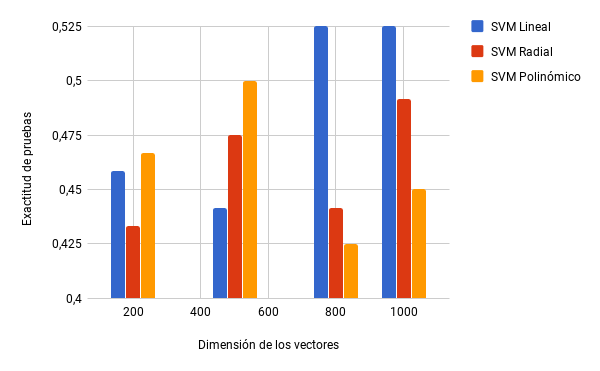
\includegraphics[width=\linewidth]{figuras/acc_svm_w2v.png}}
            %\captionsetup{justification=centering}
            \caption{Comparación del desempeño de los SVM con Word2Vec como vectorizador con distintas dimensiones de vectores.}
            \label{fig:acc_svm_w2v}
        \end{figure}
    
        Del mismo modo, el uso de un vectorizador de tipo Bag-of-Words no logró mucho como intento de mejorar el desempeño de las SVM (Figura \ref{fig:acc_svm_cv}). Esto apunta a que el pobre desempeño de las SVM como clasificador para los datos siendo utilizados puede deberse al tamaño del dataset más que al tipo de vectorizador en uso.
        
        \begin{figure}[htbp]
            \centerline{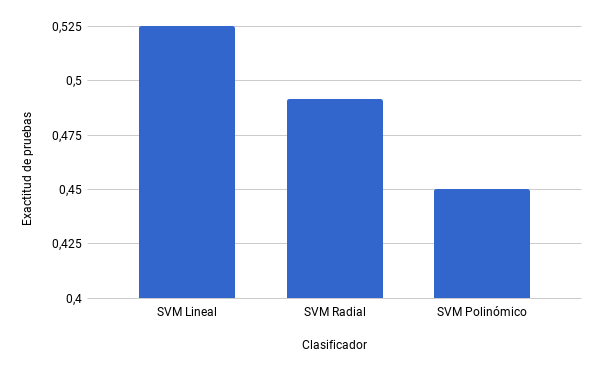
\includegraphics[width=\linewidth]{figuras/acc_svm_cv.png}}
            %\captionsetup{justification=centering}
            \caption{Comparación del desempeño de los SVM con vectorizador de tipo Bag-Of-Words.}
            \label{fig:acc_svm_cv}
        \end{figure}
    
        Por otro lado, la Red Neuronal Convolucional alcanzó la exactitud mínima en todos los casos (Figura \ref{fig:acc_rnc}), tanto para el vectorizador Word2Vec con distintos tamaños de vectores, como con el vectorizador Bag-Of-Words, con el cual se alcanzó el mejor desempeño (78,9\%), una diferencia bastante marcada respecto al uso de Word2Vec. Con lo anterior se puede inferir, entonces, que el vectorizador Word2Vec podría desempeñarse mejor si, tal como se expresa en la literatura, se utiliza un dataset con una cantidad de datos suficiente tanto para el vectorizador como para el clasificador.
        
        \begin{figure}[htbp]
            \centerline{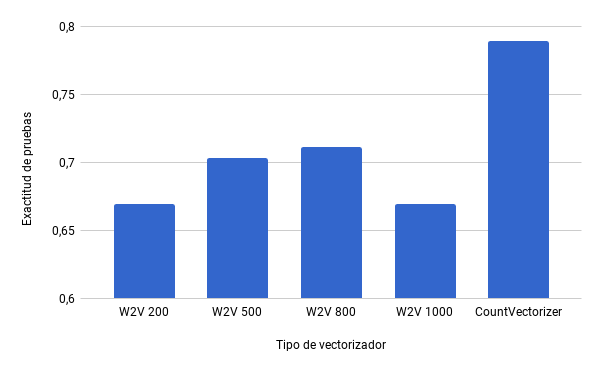
\includegraphics[width=\linewidth]{figuras/acc_rnc.png}}
            %\captionsetup{justification=centering}
            \caption{Comparación del desempeño de los vectorizadores con el clasificador de tipo Red Neuronal Convolucional.}
            \label{fig:acc_rnc}
        \end{figure}
    
        Adicionalmente, las pruebas realizadas para comparar el desempeño del vectorizador Bag-Of-Words con la Red Neuronal Convolucional, para palabras, bigramas, \textit{3}-gramas, \textit{4}-gramas y \textit{5}-gramas, muestran una ligera mejora en el desempeño del clasificador cuando se toma más información contextual de las oraciones para su vectorización --- específicamente para \textit{4}-gramas (Figura \ref{fig:acc_rnc_ngrams}). Sin embargo, el comportamiento es similar, en el caso del dataset disponible, para todos los \textit{n}-gramas tomados en consideración, lo cual puede deberse a la longitud limitada de las oraciones en la base de datos.
        
        \begin{figure}[htbp]
            \centerline{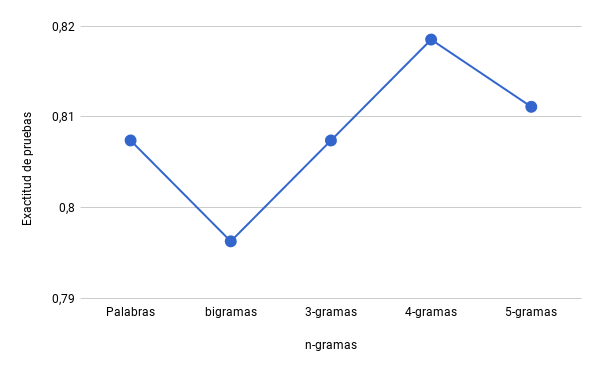
\includegraphics[width=\linewidth]{figuras/acc_rnc_ngrams.png}}
            %\captionsetup{justification=centering}
            \caption{Comparación del desempeño de las RNC con vectorizador Bag-Of-Words para distintos \textit{n}-gramas.}
            \label{fig:acc_rnc_ngrams}
        \end{figure}
    
        La Figura \ref{fig:matriz_confusion} muestra la matriz de confusión de las pruebas de la Red Neuronal Convolucional más apropiada que pudo encontrarse, utilizando \textit{4}-gramas, la cual indica, entre otras cosas, la cantidad de falsos positivos de un conjunto de clasificaciones. En esta se puede observar que, para la clase de oraciones con sentimiento \textit{neutral}, existe una discrepancia considerable, con solo un 50\% de oraciones correctamente clasificadas, lo cual puede deberse a que las personas participantes de la recolección de datos no entendieran exactamente lo que se considera un sentimiento neutral.
    
        \begin{figure}[htbp]
            \centerline{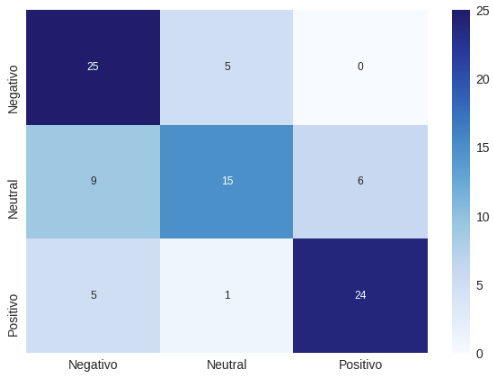
\includegraphics[width=\linewidth]{figuras/matriz_confusion.png}}
            %\captionsetup{justification=centering}
            \caption{Matriz de confusión de la evaluación del modelo de Red Neuronal Convolucional con \textit{4}-gramas.}
            \label{fig:matriz_confusion}
        \end{figure}
    
    % ------------------ FIN Resultados de los experimentos ------------------ %

% ----------------------------- FIN Experimentos ----------------------------- %

% ---------------------------------------------------------------------------- %

% ---------------------------- INICIO Conclusiones --------------------------- %

\section{Conclusiones} \label{sec:conclusiones}
    
	El objetivo de esta investigación es estudiar y comparar dos tipos de vectorizadores y dos tipos de clasificadores para la identificación de la orientación del sentimiento de documentos (texto). Las aplicaciones son bastas, siendo una de estas la implementación de detección de emociones, en un canal, para un robot social. Este canal puede ser el audio, el cual, luego se ser procesado y transformado a texto, puede ser clasificado por el módulo en cuestión.
    
    Debido a la poca cantidad de datos disponibles, fue necesario realizar pruebas con distintos tipos de vectorizadores, las cuales apuntan a que un modelo simple, como el Bag-Of-Words, se desempeña mejor para pocos datos que vectorizadores más complejos, como el Word2Vec. Del mismo modo y, probablemente por el mismo motivo, las RNC mostraron un rendimiento superior a las SVM, sobre todo cuando se toma en cuenta más información contextual en el proceso de vectorización.
    
    Se cree que, si se procede a la recaudación de más datos, siguiendo el mismo procedimiento para la recolección de los actualmente disponibles, se pueda mejorar el desempeño de los clasificadores para obtener mejores resultados. Se delega como trabajo futuro el proceso de expansión de la base de datos y el desarrollo de una aplicación que permita realizar la conversión audio-texto para sentar las bases para un módulo integrable de detección de emociones para un robot social.

% ----------------------------- FIN Conclusiones ----------------------------- %

% ---------------------------------------------------------------------------- %

% ---------------------------- INICIO Referencias ---------------------------- %

\Urlmuskip=0mu plus 1mu\relax
\bibliographystyle{IEEEtran}
\nocite{*}
\bibliography{referencias}

% ------------------------------ FIN Referencias ----------------------------- %

\end{document}
